\documentclass[a4paper,fleqn]{cas-sc}
\usepackage{fontspec}
\usepackage{xeCJK}
\setCJKmainfont{SimSun}
\setCJKsansfont{SimHei}
\usepackage[numbers,sort&compress]{natbib}
\usepackage{needspace}
\usepackage{amsmath,amssymb,booktabs,graphicx,multirow,array,tabularx,placeins,float}
\usepackage{xurl}
\graphicspath{{figs/}}
\newcolumntype{Y}{>{\raggedright\arraybackslash}X}
\renewcommand{\pm}{\mathbin{\hbox{\normalfont ±}}}
\renewcommand{\times}{\mathbin{\hbox{\normalfont ×}}}
\renewcommand{\figurename}{图}
\renewcommand{\tablename}{表}
\begin{document}
\let\WriteBookmarks\relax
\shorttitle{全局与词元级图文学习}
\shortauthors{Zang and Peng}
\title[mode=title]{晶体性质预测中的全局与词元级晶体学文本：互补性与预测级平均}
\author[1]{Huaijuan Zang}\cormark[1]
\credit{Conceptualization, Methodology, Software, Validation, Formal analysis, Writing -- original draft}
\affiliation[1]{organization={Institutional affiliation}}
\author[2]{Yunfan Peng}
\credit{Supervision, Methodology, Writing -- review and editing}
\affiliation[1]{organization={Institutional affiliation}}
\cortext[1]{通讯作者}

\begin{abstract}
晶体性质预测可以结合周期晶体图与由同一结构生成的晶体学文本。在这一设定下，晶体图编码数值几何与局部连接关系，文本则提供文档级 CLS 表示和上下文词元表示，从不同抽象层级描述结构信息。本文研究图条件余弦归一化词元注意力，并在六项 JARVIS 与四项 Materials Project 任务上独立训练全局和词元级预测器。在固定数据划分、两次独立运行和固定 0.5/0.5 预测级平均下，组合预测相对 Global 基线的宏平均 MAE 降幅约为 5.9\%；每次运行均在全部十项任务上优于 Global，并在十项任务中的九项上优于两个组成预测器。同路径对照表明，普通预测平均解释了相当一部分增益；现有证据不能证明其优于 Token-only 集成。验证集上的消息级、潜空间级和共享骨干交互研究呈现性质依赖性，因此仅作为诊断性探针，而非融合位置的受控排名。结果支持：在给定协议下，样本对齐的预测互补性是一项可复现的经验发现。
\end{abstract}
\begin{keywords}晶体性质预测 \sep 图神经网络 \sep 材料语言模型 \sep 全局文本表示 \sep 词元级表示 \sep 图--文本注意力\end{keywords}
\maketitle

\section{引言}
计算材料发现日益结合高通量电子结构计算与数据驱动候选排序，Materials Project、JARVIS、AFLOW、OQMD 和 Matminer 等数据库与工具为这一过程提供了基础设施 \citep{jain2013materialsproject,choudhary2020jarvis,curtarolo2012aflow,saal2013oqmd,ward2018matminer}。密度泛函理论为能量、电子结构和力学响应提供了系统计算途径，但在大规模化学和结构空间中反复计算仍然昂贵。学习型代理模型可以在保留决定目标性质的结构因素时提供快速估计。晶体结构天然适合表示为周期图：原子是节点，局部邻域关系是边，几何特征描述周期相互作用。CGCNN 建立了晶体图上的直接消息传递 \citep{xie2018cgcnn}；SchNet 引入连续滤波卷积 \citep{schutt2018schnet}；MEGNet 联合更新边、节点和全局状态 \citep{chen2019megnet}；ALIGNN 显式传播键角信息 \citep{choudhary2021alignn}；M3GNet 和 CHGNet 进一步发展了可迁移与预训练的原子表示 \citep{chen2022m3gnet,deng2023chgnet}。

几何并非晶体结构的唯一紧凑描述。晶体图记录原子种类、邻接关系、距离、角度和局部环境，而晶体学文本可以显式描述配位多面体、连接方式、结构维度、对称性和重复结构基元。此类文本由结构生成，因而不是独立实验模态，但它将结构信息重组为具有化学意义的抽象。图与文本在内容上部分重叠，同时在表示上有所不同：图是局部、数值化且满足置换不变性的，文本是序列化、符号化并偏向可识别概念的。二者的部分冗余使图--文本学习具有合理性，而不同抽象层级又产生了预测误差互补的可能。

Robocrystallographer 可以将晶体结构转换为可复现文本 \citep{ganose2019robocrystallographer}。Transformer 编码器 \citep{vaswani2017attention,devlin2019bert} 以及 SciBERT、MatBERT 和 MatSciBERT 等科学与材料领域适配模型，为专业术语提供上下文表示 \citep{beltagy2019scibert,walker2021matbert,gupta2022matscibert}。LLM-Prop 进一步说明结构化晶体描述可用于性质预测 \citep{rubungo2025llmprop}。CrysMMNet 和 LatticeLingo 等多模态材料模型表明结构与语言信号可以联合使用 \citep{das2023crysmmnet,munjal2024latticelingo}。常见做法是将完整词元序列压缩为全局文档表示并与图表示拼接；这种表示较为紧凑，但无法保留单个词元的可寻址性。

词元级图--文本交互可以保留细粒度语言信息，但未经归一化的交叉注意力可能受到数值尺度影响。对于投影后的图查询 $q$ 和词元键 $k_j$，标准缩放点积注意力使用 $s_j=q^\top k_j/\sqrt d$，该分数同时取决于方向和向量范数。在异构的图与语言空间中，不同范数可能产生跨度很大的 logits，使 softmax 近似 argmax。此时，有效词元数接近 1 可能反映尺度饱和，而非精确语义定位；本文不单独使用这一诊断来证明化学语义。

因此，本文的核心问题不是是否使用文本，而是文档级与词元级文本信息在图--文本晶体性质预测中应如何使用、应在何处交互。本文将全局表示定义为最大序列长度范围内的 MatBERT CLS 嵌入，将词元级表示定义为对上下文 MatBERT 词元状态进行图条件聚合所得的表示。这里的层级区分不同于原子级、子图级、分子级或晶体级表示层次；本文关注同一生成晶体学文本内部的不同抽象层级。

可能的融合位置包括消息级交互、潜空间交互、共享骨干预测融合以及独立预测级融合。CLS 向量概括完整描述，而词元状态保留位置相关的上下文证据。对二者进行压缩、门控或乘性交互，可能抑制有用的词元差异、过度强调文档背景，或使表示对性质特定相关性更加敏感。本文实验中的交互信号通常可以测量，但消息级、潜空间级和共享骨干交互比独立预测级融合表现出更强的性质依赖性。

本文将贡献定位为图--文本晶体性质预测中文档级与词元级文本表示的经验性研究。最终框架保留全局文本路径与词元级文本路径作为独立预测器，并研究其样本对齐输出及误差之间的关系。本文不预设早期融合必然更优，而是检验两种文本抽象层级是否更适合通过独立预测路径和预测级互补来利用。

本文贡献包括四点。第一，研究从冻结 MatBERT 上下文状态中提取图条件余弦归一化词元信息。第二，在主独立预测路径之外，进行受控验证集消融，在共同预测头和目标函数下比较 CLS 池化、掩码上下文词元平均池化和图条件余弦注意力。第三，通过逐样本误差、Oracle 诊断、同路径对照和固定预测级平均分析预测互补性。第四，将验证集上的消息级、潜空间级和共享骨干变体作为交互行为的诊断探针，而不对融合位置做受控排名。

\section{相关工作}
\subsection{晶体图神经网络}
晶体图神经网络可以按照消息传递中强调的几何信息进行归纳。CGCNN 从原子和键描述符学习边条件更新 \citep{xie2018cgcnn}，SchNet 通过连续滤波建模原子间距离 \citep{schutt2018schnet}，MEGNet 联合更新边、节点和全局属性 \citep{chen2019megnet}。方向模型进一步引入角度信息：DimeNet 使用径向和球面基构造方向消息 \citep{gasteiger2020dimenet}，ALIGNN 交替执行原子图和线图传播以显式建模键角 \citep{choudhary2021alignn}。NequIP 等变网络通过旋转等变约束提高原子能量与力预测的数据效率 \citep{batzner2022nequip}。Matformer 和 ComFormer 面向周期晶体构建几何 Transformer \citep{yan2022matformer,yan2024comformer}，SFTGNN 采用球谐傅里叶增强的晶体消息传递 \citep{jiang2025sftgnn}。Roost 和 CrabNet 则提供仅基于组成的结构无关参照 \citep{goodall2020roost,wang2021crabnet}。材料基础模型相关研究进一步强调可迁移原子表示和对话式多模态材料表示，包括 M3GNet、CHGNet、MACE 和 MatterChat \citep{chen2022m3gnet,deng2023chgnet,batatia2023mace,tang2025matterchat}。这些方法主要处理几何、原子或组成表示，并不直接回答图信息应如何与文档级和词元级晶体学语言表示交互。

\subsection{材料语言模型}
科学语言包含密集实体、化学式、计量约定和领域关系。材料文本还包含化学式、空间群符号、配位术语、键合描述以及结构原型和基元名称。MatBERT 和 MatSciBERT 将 Transformer 语言建模适配到材料语料，为材料术语提供上下文表示 \citep{walker2021matbert,gupta2022matscibert}。Robocrystallographer 通过从结构生成对称性、配位和连接关系描述，在结构与语言之间建立可复现接口 \citep{ganose2019robocrystallographer}。这种一致性有利于多模态学习，但生成文本仍受描述引擎的启发式规则与词汇范围限制，因此应被视为互补结构视角，而非独立真值。

\subsection{多模态材料学习}
多模态表示学习受到 CLIP、ALBEF 和 BLIP 等图像--文本模型的显著影响，它们通过对比目标、跨模态注意力和自举式图文监督建立成对模态之间的联系 \citep{radford2021clip,li2021albef,li2022blip}。这些模型说明多模态学习既可以受益于共享对齐空间，也可能需要保留模态特定表示。对于晶体性质预测，文本描述由晶体结构生成而非独立观测，因此图与文本具有部分冗余，问题转化为如何利用同一材料的不同抽象层级。

晶体多模态学习已将结构、组成、图像、谱学和文本用于性质预测或表示学习。CrysMMNet 结合晶体图和文档级语言表示，LatticeLingo 则研究局部、半全局和全局结构范围的描述 \citep{das2023crysmmnet,munjal2024latticelingo}。CAST 使用交叉注意力进行结构--文本交互，Hybrid-LLM-GNN 将图和材料语言嵌入用于跨性质预测 \citep{lee2025cast,li2025hybridllmgnn}。CLICS 探索图--文本对比学习，MatterChat 将材料多模态扩展到对话式基础模型 \citep{ozawa2024clics,tang2025matterchat}。与这些工作不同，本文聚焦于同一生成晶体学文本中的表示粒度，即文档级 CLS 与上下文词元状态，以及二者在固定基准协议下的预测互补性。

\subsection{细粒度跨模态注意力}
跨注意力通常依据 Transformer 的缩放点积注意力对两个模态的元素进行对齐 \citep{vaswani2017attention}。在材料性质预测中，图级查询与文本词元键构成自然的非对称形式：晶体查询其描述中哪些部分有用。然而，点积相似度同时包含方向和范数。当编码器和投影层的尺度统计不同，注意力尖锐度可能由范数而非对应关系决定。Query-Key Normalization 提倡对两侧投影进行归一化，以抑制任意 softmax 饱和 \citep{henry2020qknorm}。CLIP 也使用归一化图文特征与温度来稳定对齐 \citep{radford2021clip}。本文采用归一化查询--键形式，并将熵、有效词元数和最大注意力仅作为词元选择行为的诊断，而不是化学因果性的直接证据。

\section{方法}
\subsection{问题定义}
设样本为 $(G,T,y)$，其中 $G=(V,E)$ 是周期晶体图，$T=(w_1,\ldots,w_L)$ 是 Robocrystallographer 描述，$y\in\mathbb{R}$ 是标量性质。目标是学习使平均绝对误差（MAE）最小的 $f(G,T)$。本文构建两个预测器 $f_g$ 和 $f_t$，它们使用同一材料输入的不同文本抽象层级，并在输出层进行组合。

\subsection{全局与词元级预测框架}
图~\ref{fig:overall} 展示完整数据流，但不表示一个联合的潜空间融合网络。形式上，$\hat y_g=f_{\mathrm{Global}}(G,T)$ 和 $\hat y_t=f_{\mathrm{Token}}(G,T)$ 由独立训练的模型产生，检查点根据验证集选择。每个预测器包含自己的 SFTGNN 实例；二者架构相同，均使用 92 维原子输入、五层 SFTConv、128 维节点状态和平均池化，但参数不共享。全局路径读取最大序列长度内的 MatBERT CLS 状态，词元路径保留符合条件的非特殊上下文词元状态并执行图条件注意力。最终的预测级平均只作用于样本对齐的输出。需要指出的是，全局与词元预测器的比较并不能将文本粒度作为单一因果因素隔离，因为两条路径的预测头和训练目标也不同：Global 路径直接进行图--CLS 回归，Token 路径进行图条件词元聚合并使用辅助图损失。

\begin{figure}[pos=t]\centering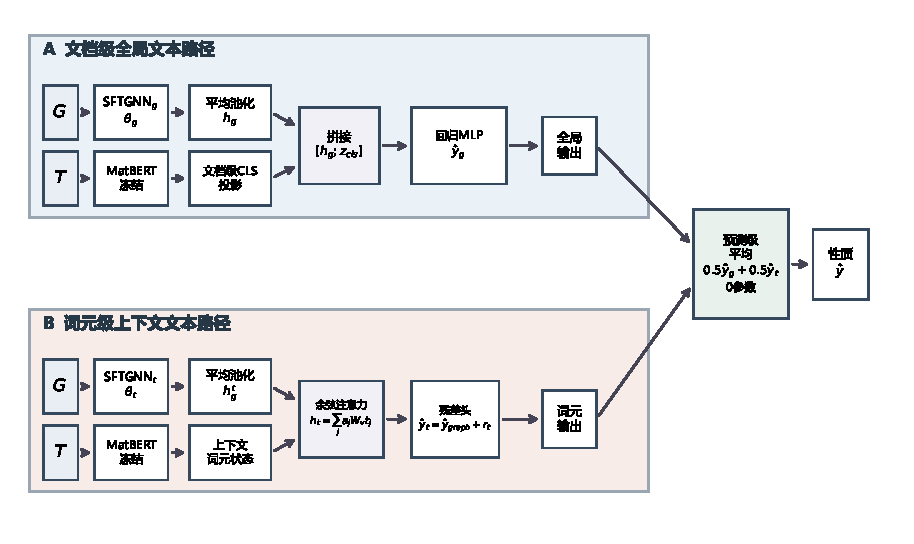
\includegraphics[width=\linewidth]{overall_framework_v9_zh.pdf}
\caption{全局与词元级图--文本学习框架。全局文本路径使用文档级 MatBERT CLS 表示，词元级路径使用图条件余弦注意力聚合上下文词元状态。两条路径在相同图编码器架构下独立训练，用于评估预测级互补性，而不引入共享潜空间交互模块。消息级、潜空间级和共享骨干交互作为诊断研究单独分析，因为其行为具有性质依赖性。}\label{fig:overall}\end{figure}

\subsection{球谐晶体图编码器}
对于边 $(j,i)$，实现从倒数距离计算径向特征 $e^r_{ij}=\mathrm{MLP}_{r}(\mathrm{RBF}(1/d_{ij}))\in\mathbb{R}^{64}$，并将球谐函数投影为 $e^s_{ij}\in\mathbb{R}^{64}$。当 $h_i,h_j\in\mathbb{R}^{128}$ 时，SFTConv 为
\begin{align}
u_{ij}&=[h_i;h_j;e^r_{ij};e^s_{ij}]\in\mathbb{R}^{384},\\
m_{ij}&=\sigma(\mathrm{MLP}_{gate}([h_i;h_j;e^r_{ij}]))\odot\mathrm{MLP}_{msg}(u_{ij}),\\
h'_i&=\mathrm{SiLU}\!\left(h_i+\mathrm{BN}\!\left(\sum_{j\in\mathcal{N}(i)}m_{ij}\right)\right).
\end{align}
两个多层感知机使用 512 维隐藏层并输出 128 维特征。五次更新后执行平均散射池化。

\begin{figure}[pos=t]\centering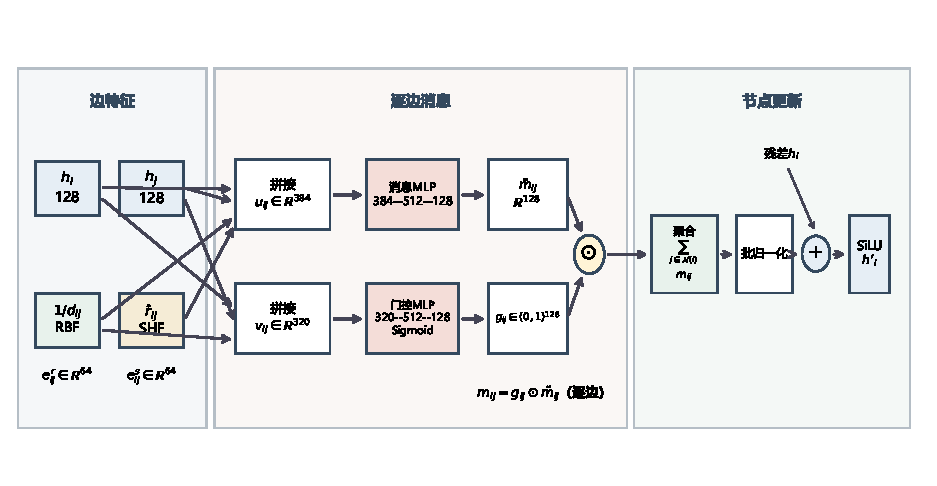
\includegraphics[width=\linewidth]{sftconv_architecture_zh.pdf}
\caption{SFTConv 消息传递，对应公式（2）：每条边上先将 Message MLP 输出与 sigmoid Gate MLP 输出逐元素相乘，再对门控消息进行邻居求和；聚合后执行批归一化、残差加法和 SiLU。}\label{fig:sft}\end{figure}

\subsection{全局文本路径}
全局路径对应本文使用的原始 SFTMAT 风格基线：将 SFTGNN 图表示与投影后的 MatBERT CLS 表示直接拼接，并输入回归头。CLS 状态 $z_{cls}\in\mathbb{R}^{768}$ 经 $768\rightarrow128\rightarrow64$ 投影和 ReLU 变换，全局预测为
\begin{equation}\hat y_g=\mathrm{MLP}_g([h_g;\phi_{cls}(z_{cls})]).\end{equation}
该路径保留文档级语义摘要。

\subsection{词元级文本路径}
MatBERT 在最大长度 128 下冻结并缓存。缓存包含形状为 $[N,128,768]$ 的最后隐状态、输入 ID 和注意力掩码，采用 BF16 存储。填充、CLS 和 SEP 位置不参与归一化注意力。保留词元身份使模型能够进行图条件选择，同时将语言模型计算移出性质模型训练循环。

\subsection{范数诱导的注意力塌缩}
原始注意力使用 $q=W_qh_g$ 和 $k_j=W_kt_j$。由于 $q^\top k_j=\|q\|\|k_j\|\cos\theta_j$，尺度与对齐无法分离。较大范数会放大微小角度差异，使 softmax 接近 one-hot。本文以熵 $H(a)=-\sum_j a_j\log a_j$ 和有效词元数 $N_{eff}=\exp(H(a))$ 量化尖锐程度。

\subsection{归一化的图条件词元注意力}
为移除范数对相似度的直接影响，本文使用
\begin{equation}
q=\frac{W_qh_g}{\|W_qh_g\|_2},\qquad k_j=\frac{W_kt_j}{\|W_kt_j\|_2},\qquad a_j=\operatorname{softmax}_{j\in\mathcal M}\!\left(\frac{q^\top k_j}{\tau}\right),
\end{equation}
其中 $\tau=0.5$，$\mathcal M$ 为有效词元集合。聚合表示为
\begin{equation}h_t^*=\mathrm{LayerNorm}\!\left(\sum_{j\in\mathcal M}a_jW_vt_j\right).\end{equation}

\begin{figure}[pos=t]\centering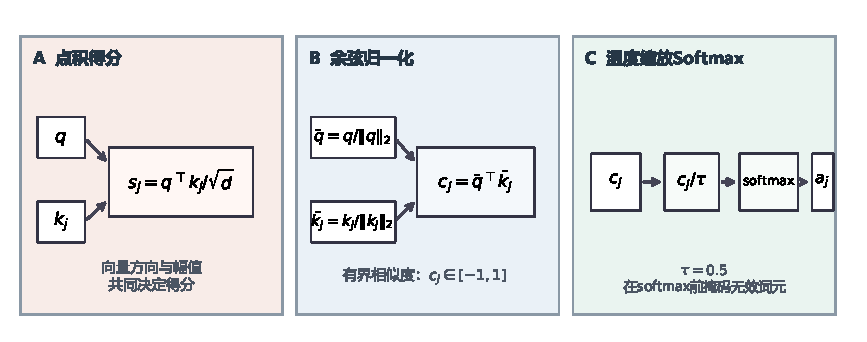
\includegraphics[width=\linewidth]{attention_temperature_zh.pdf}
\caption{图条件词元注意力机制。原始点积同时受向量方向与幅值影响，余弦归一化限制相似度范围，温度缩放 softmax 将归一化得分转化为掩码注意力权重。图中不包含实测注意力数值。}\label{fig:attention}\end{figure}

\subsection{词元级预测器}
词元路径保留显式图预测，并学习文本条件残差：
\begin{align}\hat y_{graph}&=f_{graph}(h_g),\\\Delta y&=f_r([h_g;h_t^*]),\\\hat y_t&=\hat y_{graph}+\Delta y.\end{align}
其训练损失为
\begin{equation}\mathcal L_t=\mathrm{MAE}(\hat y_t,y)+0.2\,\mathrm{MAE}(\hat y_{graph},y).\end{equation}

\subsection{预测级组合}
最终预测定义为
\begin{equation}\boxed{\hat y=\frac{\hat y_g+\hat y_t}{2}}.\end{equation}
该规则不包含可训练组合参数、任务特定权重、数据集特定路由或基于验证集的权重搜索。全局路径强调稳定的文档级摘要，词元路径强调图条件上下文词元证据。输出层组合避免将文档级与词元级表示强制压缩到共享潜空间。

\subsection{训练目标与计算复杂度}
全局路径最小化 $\mathcal L_g=|\hat y_g-y|$，词元路径使用上式 $\mathcal L_t$。两条路径独立训练，并根据最小验证 MAE 选择检查点。除图编码外，词元注意力开销为 $O(BLd_a)$，其中 $L=128$、$d_a=128$。组合预测需要同时执行两条路径，以额外推理开销换取预测性能。

\section{实验}
\subsection{数据集与任务}
本文评估六项 JARVIS 和四项 Materials Project 晶体性质预测任务，遵循 CrysMMNet 采用的基准数据准备与固定划分 \citep{das2023crysmmnet}。数据来自 JARVIS 和 Materials Project \citep{choudhary2020jarvis,jain2013materialsproject}，Matbench 提供更广泛的标准化材料基准背景 \citep{dunn2020matbench}。十项任务覆盖电子、能量和力学性质。Materials Project 的体积模量和剪切模量在训练和评估前对原始 GPa 目标应用 $\log_{10}$ 变换，因而对应 MAE 在变换后的目标空间中报告。

\subsection{文本生成与缓存}
每个晶体通过 Robocrystallographer 转换为文本，并由 MatBERT 进行分词。本文指最大序列长度内可用的分词晶体学描述，而不假定所有生成文本均被完整保留。序列最大长度为 128，并使用截断和填充掩码。全局路径读取位置零的 CLS 表示；词元路径读取完整最后隐状态，并从注意力候选中移除 CLS、SEP 和 PAD。MatBERT 表示以 BF16 预计算，并与输入 ID 和掩码配对，因此当缓存可用时，性质模型训练和推理不重复执行语言模型前向计算。

\subsection{训练协议}
主 Global、Token 和 Global+Token 实验采用两个独立的模型训练种子 42 和 43 重复运行，所有模型使用相同固定数据划分。架构、超参数、目标变换、MatBERT 序列长度、温度 $\tau=0.5$、检查点准则、固定 0.5/0.5 预测级平均和测试协议均不变。每次运行中，全局文本预测器和词元级文本预测器均独立初始化和训练，批大小为 32，评估批大小为 64；优化器为 AdamW \citep{loshchilov2019adamw}，学习率和 OneCycleLR 最大学习率为 $10^{-3}$，权重衰减为 $10^{-4}$，使用 BF16 自动混合精度，训练预算为 300 轮。每个预测器按最小验证 MAE 选择，随后测试集仅评估一次。预测按样本 ID 对齐，目标在浮点精度内一致后再平均；带隙输出裁剪为非负值。交互位置研究属于验证集诊断实验，任务和运行覆盖范围见第 5.5 节，并未统一采用主测试协议的两次重复。

为隔离文本表示与路径特定预测头和训练目标的影响，本文还在覆盖 JARVIS 与 Materials Project 电子、能量和力学性质的平衡六任务子集上进行单种子匹配验证消融。CLS、掩码平均和余弦注意力变体使用相同图编码器、128 维文本输出、回归头、MAE 目标、优化器、调度器、训练预算、验证划分和训练种子 42，仅改变 MatBERT 表示的聚合方式。该结果仅用于文本表示层级分析，不在测试集上评估。

\subsection{评估指标}
MAE 是主要指标，因为它位于基准目标空间中并可限制极端误差的影响。相对 Global 的增益定义为 $(\mathrm{MAE}_g-\mathrm{MAE}_{dual})/\mathrm{MAE}_g\times100\%$。此外，本文报告绝对误差 Pearson 相关性、Oracle MAE 和验证集逐样本胜出比例。模型选择和固定 0.5/0.5 规则仅使用验证集，测试集不参与训练、调参或检查点选择。

两次运行的验证预测还定义了同路径对照。令 $G_1,G_2$ 为种子 42 和 43 的 Global 预测，$T_1,T_2$ 为 Token 预测，计算 $GG=(G_1+G_2)/2$、$TT=(T_1+T_2)/2$，并与运行匹配的 $GT_1=(G_1+T_1)/2$、$GT_2=(G_2+T_2)/2$ 比较。每个任务的四个文件具有相同的样本 ID 集合和顺序，目标的最大绝对数值差异为 $2.39\times10^{-7}$。不从验证标签拟合任何预测权重。

\section{结果}
\subsection{总体性能}
表~\ref{tab:test}报告两次独立运行的测试集 MAE 均值、样本标准差和相对 Global 的增益。十项任务每次运行合计包含 24,671 个样本--任务评估，并不等于不同晶体的数量。预测级组合在两次运行的全部十项任务上均优于 Global，平均宏相对 MAE 降幅约为 $5.9\%$（两次运行均值 $\pm$ 样本标准差为 $5.875\pm0.036\%$）。该小标准差仅用于说明两次运行的一致性，不作为正式显著性检验。在每次运行中，组合预测还在十项任务中的九项上同时优于两个单独路径。每次运行有一项任务由 Token 略微取得更低 MAE，但组合仍优于对应 Global 路径。相对 Global，JARVIS 和 Materials Project 的平均宏增益分别为 $5.747\pm0.069\%$ 和 $6.068\pm0.193\%$。

两次运行的宏相对 MAE 降幅分别为 5.850\% 和 5.901\%，说明总体收益接近。按两次运行的任务均值计算，组合预测在电子性质上的 MAE 降低 3.011--7.204\%，在能量性质上降低 6.576--7.736\%，在力学性质上降低 3.400--7.092\%。

\begin{table}[!htbp]\caption{两次独立运行的测试集 MAE 及相对 Global 的增益。数值为均值 $\pm$ 样本标准差；MAE 越低越好。粗体表示相同评估协议下的最佳结果，下划线表示次优结果。}\label{tab:test}\centering\scriptsize
\resizebox{\linewidth}{!}{\begin{tabular}{lrrrr}\toprule 任务&Global&Token&Global+Token&增益（\%）\\\midrule
JARVIS-MBJ&\underline{0.259641 $\pm$ 0.002825}&0.267325 $\pm$ 0.009433&\textbf{0.251800 $\pm$ 0.001808}&3.011 $\pm$ 1.752\\
JARVIS-OPT&0.124654 $\pm$ 0.003559&\underline{0.119036 $\pm$ 0.004411}&\textbf{0.115764 $\pm$ 0.000876}&7.104 $\pm$ 1.950\\
JARVIS-Formation&0.029453 $\pm$ 0.000692&\underline{0.028832 $\pm$ 0.000190}&\textbf{0.027437 $\pm$ 0.000406}&6.836 $\pm$ 0.810\\
JARVIS-Total&0.032296 $\pm$ 0.000405&\underline{0.031422 $\pm$ 0.000010}&\textbf{0.029796 $\pm$ 0.000167}&7.736 $\pm$ 0.639\\
JARVIS-Bulk&9.60549 $\pm$ 0.14011&\underline{9.40847 $\pm$ 0.09234}&\textbf{9.14175 $\pm$ 0.04797}&4.821 $\pm$ 0.889\\
JARVIS-Shear&8.96774 $\pm$ 0.03243&\underline{8.72852 $\pm$ 0.12811}&\textbf{8.52204 $\pm$ 0.13611}&4.972 $\pm$ 1.174\\
MP-Bandgap&0.211599 $\pm$ 0.003322&\textbf{0.196220 $\pm$ 0.002127}&\underline{0.196354 $\pm$ 0.002946}&7.204 $\pm$ 0.065\\
MP-Formation&0.024373 $\pm$ 0.000796&\underline{0.024256 $\pm$ 0.000511}&\textbf{0.022769 $\pm$ 0.000646}&6.576 $\pm$ 0.399\\
MP-Bulk&0.037610 $\pm$ 0.001028&\underline{0.036156 $\pm$ 0.000402}&\textbf{0.034938 $\pm$ 0.000623}&7.092 $\pm$ 0.884\\
MP-Shear&0.071981 $\pm$ 0.000318&\underline{0.071636 $\pm$ 0.000668}&\textbf{0.069533 $\pm$ 0.000013}&3.400 $\pm$ 0.445\\\midrule
宏平均增益&&&&5.875 $\pm$ 0.036\\\bottomrule\end{tabular}}\end{table}

\subsection{与现有方法的比较}
表~\ref{tab:jarvis_lit} 和表~\ref{tab:mp_lit} 给出不同数据划分、目标变换和测试协议下的文献参照。由于各研究的协议不一致，这些结果仅用于背景参照，不构成协议匹配的跨研究排名。本文的主要结论均来自内部复现且样本对齐的比较。

\begin{table}[pos=H]\caption{不同协议下 JARVIS 上的文献参照比较。形成能和总能量单位为 eV/atom，带隙为 eV，弹性模量为 GPa。已发表数值沿用各研究的评估协议；粗体和下划线仅用于列内视觉参照，不表示协议匹配的跨研究排名。}\label{tab:jarvis_lit}\centering\scriptsize
\resizebox{\linewidth}{!}{\begin{tabular}{lrrrrrr}\toprule 方法&形成能&Bandgap OPT&Bandgap MBJ&总能量&Bulk $K_v$&Shear $G_v$\\\midrule
CGCNN&0.063&0.200&0.413&0.078&14.47&11.75\\SchNet&0.045&0.192&0.433&0.047&14.33&10.67\\MEGNet&0.047&0.145&0.344&0.058&15.11&13.09\\GATGNN&0.047&0.170&0.513&0.056&14.32&12.48\\ALIGNN&0.033&0.142&0.310&0.037&10.40&9.481\\Matformer&0.0325&0.137&0.300&0.035&--&--\\PotNet&0.0294&0.127&0.272&0.032&--&--\\CrysMMNet&0.028&0.128&0.278&0.034&\underline{9.625}&\textbf{8.471}\\eComFormer&0.0284&0.124&0.280&0.032&--&--\\iComFormer&\textbf{0.0272}&\underline{0.122}&\underline{0.260}&\textbf{0.0288}&--&--\\SFTGNN&0.0283&0.129&0.270&0.031&--&--\\本文（Global+Token）&\underline{0.027437}&\textbf{0.115764}&\textbf{0.251800}&\underline{0.029796}&\textbf{9.14175}&\underline{8.52204}\\\bottomrule\end{tabular}}\end{table}

\begin{table}[pos=H]\caption{不同协议下 Materials Project 上的文献参照比较。形成能单位为 eV/atom，带隙为 eV，弹性模量为 $\log_{10}(\mathrm{GPa})$。已发表数值沿用各研究的评估协议；粗体和下划线仅用于列内视觉参照，不表示协议匹配的跨研究排名。}\label{tab:mp_lit}\centering\scriptsize
\resizebox{\linewidth}{!}{\begin{tabular}{lrrrr}\toprule 方法&形成能&带隙&Bulk moduli&Shear moduli\\\midrule
CGCNN&0.031&0.292&0.047&0.077\\SchNet&0.033&0.345&0.066&0.099\\MEGNet&0.030&0.307&0.060&0.099\\GATGNN&0.033&0.280&0.045&0.075\\ALIGNN&0.022&0.218&0.051&0.078\\Matformer&0.021&0.211&0.043&0.073\\PotNet&0.0188&0.204&0.040&0.0650\\CrysMMNet&0.020&0.197&0.038&\textbf{0.062}\\eComFormer&\textbf{0.01816}&0.202&0.0417&0.0729\\iComFormer&\underline{0.01826}&\textbf{0.193}&0.0380&\underline{0.0637}\\SFTGNN&0.0183&0.198&\underline{0.037}&0.064\\本文（Global+Token）&0.022769&\underline{0.196354}&\textbf{0.034938}&0.069533\\\bottomrule\end{tabular}}\end{table}

\subsection{匹配的文本表示消融}
为隔离文本表示的影响，本文在平衡六任务子集上比较三种聚合方式。该子集覆盖两个数据集和三类性质：JARVIS-Bandgap\_MBJ、JARVIS-FormationEnergy、JARVIS-BulkModulusKv、MP-Bandgap、MP-FormationEnergy 和 MP-ShearModuli。三种变体使用相同 SFTGNN 图编码器、128 维文本输出、回归头、MAE 目标、优化器、调度器、训练预算、验证划分和种子 42，仅改变 MatBERT 序列的表示方式：CLS 状态、对有效上下文词元进行掩码平均，或图条件余弦注意力。

\begin{table}[H]\caption{平衡六任务子集上的匹配文本表示验证消融。MAE 越低越好；粗体表示最佳结果，下划线表示次优结果。归一化宏平均按任务相对于 CLS 计算，不是原始 MAE 的直接平均。}\label{tab:matched_text}\centering\scriptsize
\begin{tabular}{lrrr}\toprule 任务&CLS&掩码平均&余弦注意力\\\midrule
JARVIS-MBJ&\underline{0.246605}&\textbf{0.236364}&0.260371\\JARVIS-Bulk&\textbf{8.971401}&9.361474&\underline{9.061776}\\JARVIS-Formation&\textbf{0.029189}&\underline{0.029192}&0.029690\\MP-Bandgap&0.217180&\underline{0.216474}&\textbf{0.214222}\\MP-Formation&\underline{0.020157}&\textbf{0.019904}&0.020422\\MP-Shear&\textbf{0.069412}&\underline{0.069488}&0.075792\\\midrule
归一化宏平均&\underline{1.0000}&\textbf{0.9979}&1.0291\\\bottomrule\end{tabular}\end{table}

六项匹配任务中没有一种文本表示占据统一优势：CLS、掩码平均和余弦注意力分别在 3、2 和 1 项任务上取得最低验证 MAE。归一化宏平均分别为 1.0000、0.9979 和 1.0291。因此，上下文词元状态可以帮助部分性质，但在匹配设定下余弦注意力并不普遍更优。该单种子验证消融不替代主实验的两次测试运行。

余弦归一化从相似度中移除查询与键的范数影响，使温度 $\tau$ 成为显式的尖锐度控制量。现有验证诊断显示注意力较为分散而非集中于单一词元，但这些统计只刻画注意力行为，不能证明普遍预测收益或化学因果性。

\subsection{全局与词元级表示的互补性}
\begin{table}[pos=H]\caption{单独预测器以及同视角和跨视角预测组合的验证性能。数值为两次独立运行的平均验证 MAE；Global+Global 和 Token+Token 分别在同一路径的两次运行间平均预测，Global+Token 为运行匹配的跨视角平均。粗体为最佳结果，下划线为次优结果。归一化宏平均按 Global 逐任务计算。}\label{tab:validation_controls}\centering\scriptsize
\resizebox{\linewidth}{!}{\begin{tabular}{lrrrrr}\toprule 任务&Global&Token&Global+Global&Token+Token&Global+Token\\\midrule
JARVIS-MBJ&0.238892&0.247418&\textbf{0.230477}&0.235945&\underline{0.232514}\\JARVIS-OPT&0.123269&0.123004&\textbf{0.117583}&0.118742&\underline{0.117690}\\JARVIS-Formation&0.029294&0.028961&0.027565&\textbf{0.027346}&\underline{0.027449}\\JARVIS-Total&0.030939&0.030464&0.028922&\textbf{0.028319}&\underline{0.028642}\\JARVIS-Bulk&9.113950&9.128360&\underline{8.802365}&8.806866&\textbf{8.798694}\\JARVIS-Shear&8.652951&8.577900&8.397938&\textbf{8.335904}&\underline{8.343903}\\MP-Bandgap&0.213246&0.209270&0.202748&\textbf{0.199835}&\underline{0.201250}\\MP-Formation&0.020522&0.019973&0.019189&\textbf{0.018730}&\underline{0.018892}\\MP-Bulk&0.037887&0.036314&0.036431&\textbf{0.035190}&\underline{0.035667}\\MP-Shear&0.066456&0.064897&0.064436&\underline{0.063536}&\textbf{0.063134}\\\midrule
十任务归一化宏平均&1.0000&--&0.9548&\textbf{0.9464}&\underline{0.9476}\\\bottomrule\end{tabular}}\end{table}

表~\ref{tab:validation_controls} 显示，Global 与 Token 在不同任务上表现不同，而固定跨视角平均在两次运行均值层面十项任务上都低于两个组成预测器。然而，同路径集成也能带来显著收益：Token+Token 的归一化宏 MAE 为 0.9464，略低于 Global+Token 的 0.9476。因此，普通预测平均解释了观察到收益的相当一部分，现有对照不能将全部收益唯一归因于跨视角差异。

\begin{figure}[pos=H]\centering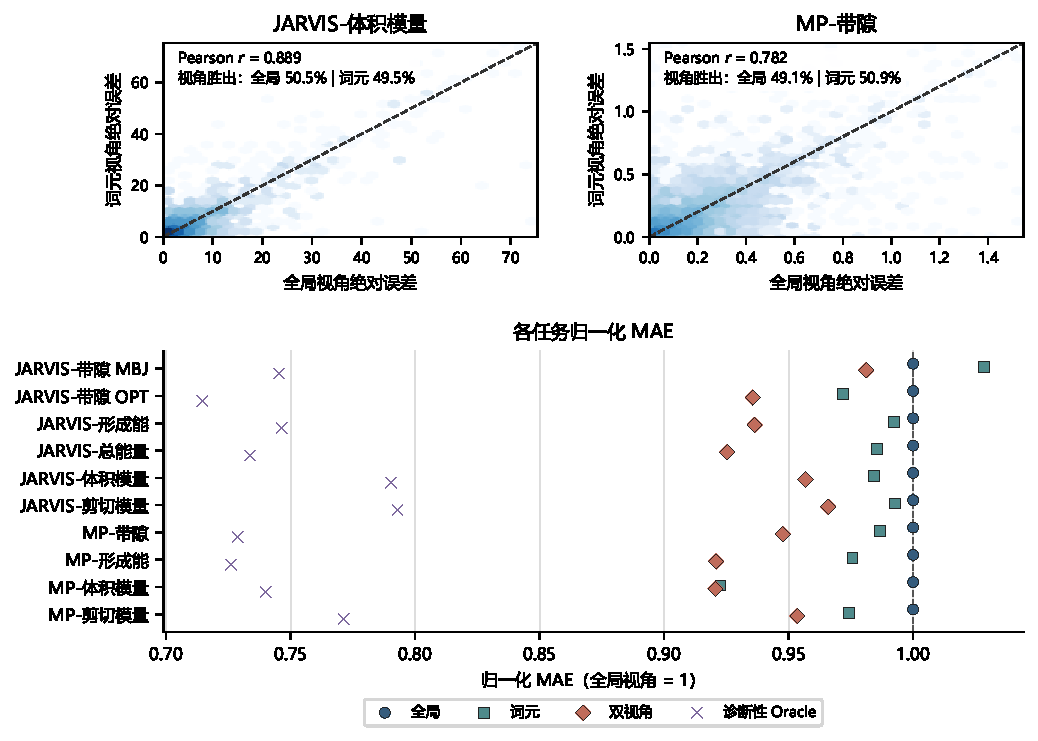
\includegraphics[width=\linewidth]{error_complementarity_zh.pdf}
\caption{代表性逐样本误差互补性分析。上方为两个代表任务的六边形分箱密度图，包含 $y=x$、Pearson $r$ 和 Global/Token 路径胜出比例；下方为十项任务中 Global、Token、固定预测级组合和诊断性 Oracle 的归一化 MAE。Oracle 使用真实标签，不可部署；图中展示一次代表性运行，两次运行的定量范围见表~\ref{tab:comp}。}\label{fig:comp}\end{figure}

\begin{table}[H]\caption{十项任务验证集互补性诊断的运行范围。胜出比例的分母包含平局。}\label{tab:comp}\centering\small
\begin{tabular}{lcc}\toprule 诊断指标&运行 1 范围&运行 2 范围\\\midrule
绝对误差 Pearson 相关性&0.614--0.900&0.591--0.906\\Oracle 相对 Global 增益（\%）&20.709--28.546&20.978--28.801\\Global 样本胜出比例（\%）&17.732--48.526&15.147--48.780\\Token 样本胜出比例（\%）&22.565--81.551&16.960--52.316\\组合相对 Global 增益（\%）&1.886--7.935&2.537--7.971\\\bottomrule\end{tabular}\end{table}

\subsection{探索性交互诊断}
本文评估验证集上的潜空间级、消息级和共享骨干变体。由于这些实验的任务覆盖、参照基线和计算预算并不统一，本文将其解释为机制探针，而不是融合位置的受控排名。潜空间查询条件化、特征细化和显式成对耦合均能改变表示，但预测效果随任务和数据集变化。SEC-SFT 的文本条件消息调制改善了若干 JARVIS 任务，却使 Materials Project 的部分力学任务退化；残差形式修复了部分退化，但不能普遍保留收益。共享骨干双视角融合在平衡六任务子集上固定平均改善 4/6 项任务，且在 5/6 项任务上低于更好的共享分支。总体而言，早期交互是可行的，但具有性质依赖性，详细诊断见附录。

\subsection{计算成本}
Global 和 Token 预测器分别包含 2,661,154 和 2,800,739 个可训练参数，保留两个独立预测器时合计为 5,461,893 个参数。固定预测级平均不增加可训练参数，但推理需要同时执行两条图--文本路径。Global 使用 CLS 表示，Token 保留缓存的上下文词元状态。

\section{讨论}
本文结果围绕三个相互关联的问题展开。第一，文档级 CLS 与上下文词元表示是否包含不同的预测信息？二者误差正相关但低于 1，并存在显著 Oracle 间隙。固定预测级平均在两次运行中均改善全部十项测试任务，相对于两个组成预测器在每次运行的九项任务上更优。匹配表示消融进一步表明，这种互补性并不能归结为某一种普遍更优的文本聚合器，因为 CLS、掩码平均和余弦注意力在共同头部与损失下分别赢得不同性质。

第二，观察到的收益是否完全来自跨视角表示互补？同路径对照显示普通预测平均贡献显著：GG 与 TT 均能降低误差。GT 优于 GG，但在归一化宏平均上不优于 TT，因此全部收益不能唯一归因于跨视角多样性。

第三，为什么保留独立预测路径而不是进行更早的交互？验证集上的潜空间、消息级和共享骨干诊断具有性质依赖性，并未提供统一改进。因此，在主协议下保留独立预测平均作为主要经验配置，但不据此声称融合位置存在普遍排名。

\section{局限性}
当前评估使用两次独立运行，可以支持一致性判断，但不能进行正式显著性检验；同路径对照也表明普通平均具有实质作用。主 Global/Token 比较同时改变文本抽象层级、预测头和训练目标；匹配的 CLS/平均/余弦消融仅在一个种子和六项验证任务上部分隔离了表示选择，不能替代完整的两次主实验。

公开基准使用不同数据划分和目标变换。双预测器设计增加存储和推理成本，本文没有在统一硬件协议下测量缓存生成、墙钟时间、延迟和峰值内存。Robocrystallographer 描述继承其生成过程的范围与启发式规则，其他中间文本抽象层级仍未研究。

交互研究仅在验证集上进行，任务覆盖不均，且未用于测试时模型选择。聚合注意力统计不能证明化学因果性或逐样本可解释性；本文也没有匹配的原始点积与余弦归一化性能消融，因此将归一化视为数值控制，而非因果性能主张。

\section{结论}
本文研究图--文本晶体性质预测中的文档级与词元级文本表示。两个独立训练的 SFTGNN--MatBERT 路径采用固定 0.5/0.5 预测级平均。在十项 JARVIS 和 Materials Project 任务、两次训练运行中，组合预测在每项任务上均优于 Global，平均宏相对 MAE 降幅约为 $5.9\%$（$5.875\pm0.036\%$），并在每次运行的十项任务中的九项上优于两个组成预测器。

匹配的六任务验证消融表明，CLS、掩码平均和余弦注意力分别受到不同性质偏好，同路径集成则说明普通预测平均解释了相当一部分收益。更早的潜空间、消息级和共享骨干交互同样具有性质依赖性。因此，本文支持的主要结论是给定协议下样本对齐的预测互补性，而不是某一种文本表示或融合位置普遍更优。

\appendix
\setcounter{topnumber}{5}\setcounter{bottomnumber}{5}\setcounter{totalnumber}{10}
\renewcommand{\topfraction}{0.95}\renewcommand{\bottomfraction}{0.95}\renewcommand{\textfraction}{0.05}\renewcommand{\floatpagefraction}{0.10}
\section{事后描述性同路径分析}
该分析使用已保存的测试预测，不用于选择架构或融合权重。对于任务 $j$，GG 和 TT 分别在两次运行间平均预测，GT 先构造运行内 Global--Token 平均。归一化宏平均为 Global $=1.000000$、GG $=0.956587$、TT $=0.935789$、GT $=0.941171$；GT 在 10 项任务中的 9 项低于 GG，但仅在 3 项低于 TT。5.8829\% 与 5.8754\% 的差异仅来自聚合顺序。

\section{潜空间交互诊断}\label{app:latent}
这些验证集变体用于探测不同潜空间交互机制，并非候选最终模型。TAGIF 表示 Token-Anchored Global Innovation Fusion，GCTA 表示 CLS 条件化图--词元注意力，GCTR 表示 CLS 条件化词元细化，PVIN 表示 Parallel-View Interaction Network。表~\ref{tab:latent_detail} 汇总具有代表性的诊断，包括交互已激活但预测作用较弱或具有性质依赖性的情况。
\begin{table}[!htbp]\caption{潜空间交互变体的验证集诊断。所有数值均来自验证集；这些变体不进行测试评估。}\label{tab:latent_detail}\centering\scriptsize
\resizebox{\linewidth}{!}{\begin{tabular}{lllll}\toprule 方法&任务&预测结果&表示或注意力诊断&语义/控制证据\\\midrule
TAGIF&JARVIS-Bandgap\_MBJ&相对 Token-only 的两任务宏增益 $-0.975\%$&innovation ratio 0.989；interaction ratio 0.432&正确 CLS 控制在两任务均优于 shuffled/zero\\
TAGIF&MP-Bandgap&相对 Token-only 获胜 0/2&innovation ratio 0.834；interaction ratio 0.695&正交分量未塌缩\\
GCTA&JARVIS-Bandgap\_MBJ&验证 MAE 0.285429，对比 naive concat 的 0.286644&$\|q_c\|/\|q_g\|=0.440$；注意力 L1 变化 0.00218&$W_{qc}$ 梯度活跃\\
GCTA&MP-Bandgap&验证 MAE 0.217874，对比 0.219016&$\|q_c\|/\|q_g\|=0.194$；注意力 L1 变化 0.00161&$W_{qc}$ 梯度活跃\\
GCTR&JARVIS-Bandgap\_MBJ&相对 naive concat 退化 0.758\%&$\cos(h_t,h_{refined})=0.968$；细化比 0.028&FiLM 分支活跃\\
GCTR&MP-Bandgap&相对 naive concat 改善 1.835\%&$\cos(h_t,h_{refined})=0.856$；细化比 0.016&语义控制不稳定\\\bottomrule\end{tabular}}\end{table}

\section{消息级交互诊断}\label{app:message}
SEC-SFT 将文本条件调制引入最终 SFTConv 消息构造；残差形式向原始消息添加零初始化的文本条件修正。下表保留第 5.5 节所述任务覆盖下的验证值。
\begin{table}[!htbp]\caption{消息级验证诊断。（a）为 SEC-SFT 的逐任务相对变化；（b）为选定的 Residual SEC-SFT 比较。所有数值均为验证结果。}\label{tab:message_detail}\centering\scriptsize
\textit{（a）SEC-SFT 逐任务相对变化}\par\smallskip
\begin{tabular}{lr}\toprule 任务&相对变化（\%）\\\midrule
JARVIS-MBJ&+1.283\\JARVIS-OPT&+0.660\\JARVIS-Formation&-1.121\\JARVIS-Total&+1.740\\JARVIS-Bulk&+2.418\\JARVIS-Shear&+2.279\\MP-Bandgap&+2.206\\MP-Formation&+1.675\\MP-Bulk&-3.844\\MP-Shear&-5.553\\\bottomrule\end{tabular}
\par\vspace{6pt}\textit{（b）Residual SEC-SFT 选定案例}\par\smallskip
\begin{tabular}{lrrr}\toprule 任务&Original&SEC-SFT&Residual SEC-SFT\\\midrule
MP-Bulk&0.03789499&0.03935185&0.03717689\\MP-Shear&0.06582852&0.06948390&0.06564737\\JARVIS-Bulk&9.2148&8.9920&9.3033\\\bottomrule\end{tabular}\end{table}

\section{共享骨干预测诊断}\label{app:shared}
共享骨干双视角融合使用一个共享 SFTGNN 编码器和两个文本预测头。下表报告平衡六任务子集上的详细验证诊断。
\begin{table}[!htbp]\caption{平衡六任务子集上的共享骨干验证诊断。}\label{tab:sbdvf_detail}\centering\scriptsize
\begin{tabular}{lrrr}\toprule 任务&绝对误差相关性&Oracle 增益（\%）&梯度余弦\\\midrule
JARVIS-MBJ&0.941&13.010&+0.477\\JARVIS-Formation&0.988&9.381&-0.435\\JARVIS-Bulk&0.987&6.273&+0.956\\MP-Bandgap&0.929&11.582&+0.476\\MP-Formation&0.981&10.755&-0.215\\MP-Shear&0.958&10.140&+0.690\\\bottomrule\end{tabular}\end{table}
\begin{table}[!htbp]\caption{平衡六任务子集上的共享骨干双视角验证诊断。数值为 MAE，增益相对匹配验证基线计算。}\label{tab:sbdvf_compact}\centering\scriptsize
\begin{tabular}{lrrrrr}\toprule 任务&Original&Shared Global&Shared Token&Final&增益（\%）\\\midrule
JARVIS-MBJ&0.240074&0.247644&0.244046&0.241591&-0.632\\JARVIS-Formation&0.028966&0.028823&0.028645&0.028505&+1.591\\JARVIS-Bulk&9.214838&8.939804&8.887833&8.869501&+3.748\\MP-Bandgap&0.212996&0.204922&0.202905&0.200832&+5.711\\MP-Formation&0.020460&0.020200&0.020050&0.019905&+2.712\\MP-Shear&0.065829&0.066835&0.068522&0.066976&-1.744\\\midrule
宏平均增益&&&&&+1.898\\\bottomrule\end{tabular}\end{table}

\FloatBarrier
\section*{致谢}
作者感谢课题组成员的讨论，并感谢 JARVIS、Materials Project、Robocrystallographer 和 MatBERT。
\section*{资助声明}
本研究未获得公共、商业或非营利机构的专项资助。
\section*{数据可用性}
本文使用的源数据可从 JARVIS 和 Materials Project 公开获取；支持本文结论的衍生描述和预测文件将在最终发布时提供。
\section*{代码可用性}
模型与分析代码将在最终发布时提供。
\section*{利益冲突声明}
作者声明不存在利益冲突。
\bibliographystyle{elsarticle-num}
\bibliography{cas-refs}
\end{document}
